%\documentclass[12pt,twocolumn]{article}
\documentclass[12pt]{article}
\usepackage[utf8]{inputenc}
\usepackage{amsmath}
\usepackage{listings}
\usepackage{graphicx}
\title{CS 472 Fall 2011 \\
     Project 2.2}
\author{Colby Blair}
\date{Due October 17th, 2011}

\begin{document}
\maketitle

\begin{abstract}
In computer science, one area of study is that of optimizing functions. There are many methods for optimization, and this repor will talk about Genetic Programming (GP). Genetic Programming creates mathematical expression trees, and modifies them to make educated guesses. They are useful for finding the function defintions for curves on a graph. 

This report presents a GP with mathematical non-terminal symbols '+', '-', '*', and '/', and terminal values as contants and variables. Although very simple, this report setups a proof of concept GP for later reports. It talks about the crossover and selection functions, as well as the population representation. It also shows two trees before and after crossover, a sample tree over different values, and finally, the code used.
\end{abstract}

\pagebreak

\tableofcontents
\listoffigures

\pagebreak

\part{Representation Description}
GPs are used to try to approximate a mathamatical expression \textbf{tree} (Section \ref{sec:trees}) that describes a function on a graph. In order to improve the approximation, a random set of expression trees are generated. This set is called the \textbf{population} (Section \ref{sec:population}). 

\section{Trees}
\label{sec:trees}
\begin{figure}[!h]
        \begin{center}
		\scriptsize
		\begin{lstlisting}
	+---------------+
	|tree		|
	|tree_node *tnp=|------------------------------ +---------------+
	|...		|				|tree_node	|
	|int nchildren= |				|enum node_type	|
	| 2 (nonterminal)|				|double dval	|
	|tree *children[]|------			|double variable*|
	+---------------+	|			+---------------+
				|
				... (many more non-terminals)
		----------------|
		|		|
		|	+---------------+
		|	|tree		|
		|	|tree_node *tnp=|-------------- +---------------+
		|	|...		|		|tree_node	|
		|	|int nchildren= |		|enum node_type	|
		|	| 0 (terminal)	|		|double dval	|
		|	|tree *children[]|--NULL	|double variable*|
		|	+---------------+		+---------------+
	+---------------+
	|tree		|
	|tree_node *tnp=|------------------------------ +---------------+
	|...		|				|tree_node	|
	|int nchildren= |				|enum node_type	|
	| 0 (terminal)	|				|double dval	|
	|tree *children[]|-------NULL			|double variable*|
	+---------------+				+---------------+
		\end{lstlisting}
		\normalsize
               \caption{An expression tree (one per individual)}
                \label{tree_rep}
        \end{center}
\end{figure}

A tree is simply class, that has pointers to child trees. Since our operators ('+', '-', '*', and '/') only take a left hand and right hand expressions, each tree only needs at most 2 children. But more or less can be inserted for future operators, on a per-operator basis. Since a tree simply points to other subtrees, the term \textbf{tree} in this report can mean either the whole tree or a subtree.

Our operators are called \textbf{non-terminals}, since they rely on the results of child subtrees to compute their results. Our \textbf{terminals} then are either constants or pointers to elements in a variable array (double, or decimal, values). Both are initialized randomly from their respective sets.

Each tree class instance points to a tree\_node class. This class holds the enumerable type of the tree class; either 'plus', 'minus', 'multi', or 'div' for non-terminal trees (operators), or 'tree\_double' or 'tree\_variable' for terminal trees.

The terminal trees will be, in future projects, mutated using point mutation, but for now are left alone. The non-terminal trees are mutated by simple regenerating a random tree in place, and selected at random. Trees of type tree\_var are, again, pointers to a variable array. This tree's value is initialized to point to a random element in the variable list. Since they are pointers, modifying variable values takes immediate affect throughout the tree. The variables in the variable array can be modified, and the tree evaluation and fitness functions (re)ran. 

\section{Population}
\label{sec:population}
In order to optimize lots of trees to reach an approximate solution


\part{Functions and Generators}
\section{Fitness Function}
\begin{figure}[!h]
        \begin{center}
		\begin{tabular}{r l}
			$ f_i(expected) $		&	$ = $ Error \\
								&	$ = | eval_i() - exptected | $ \\
								& where \\
								& $ eval_i() $ is the evaluation function in Figure \ref{eval_func}\\
		\end{tabular}
               \caption{Fitness function}
                \label{fit_func}
        \end{center}
\end{figure}

\begin{figure}[!h]
        \begin{center}
		\begin{tabular}{r l}
			$ eval_i() $	&	$ = \sum_{x=1}^{n} eval_{child_x}() $	if $i$ type is 'plus'\\
						&	$ = eval_{child_1}() - eval_{child_2}() - ... eval_{child_n}()$ if $i$ type is 'minus'\\
						&	$ = \prod_{x=1}^{n} eval_{child_x} $	if $i$ type is 'plus'\\
						&	$ = eval_{child_1}() / eval_{child_2}() / ... eval_{child_n}()$ if $i$ type is 'div'\\
						&	$ = i_{constant value} $ if $i$ type is 'tree\_double' \\
						&	$ = i_{variable valu} $ if $i$ type is 'tree\_var' \\
						& where \\
						& $ n $ is the number of children (0 or 2 only for now)
		\end{tabular}
               \caption{Evaluation function}
                \label{eval_func}
        \end{center}
\end{figure}

\pagebreak

\section{Random Tree Generator}
\begin{figure}[!h]
        \begin{center}
		\scriptsize
		\begin{lstlisting}
if random_value in 0...9 equals 0 or at depth 0:
	set this subtree to a terminal type; a randomly a contant or 
		a variable
else:
	set this subtree to a nonterminal type; randomly a 'plus', 
		'minus','multi','div'
	create each child from rand_tree_generator(depth - 1)
		\end{lstlisting}
		\normalsize
               \caption{Random tree generator}
                \label{rand_tree_gen}
        \end{center}
\end{figure}

The random tree generator generator is a recursive function that tries to construct a semi-inbalanced tree. There is a 1 in 10 chance that it will make any node not at the max depth a terminal, which leads to a moderately imbalanced tree. See Section \ref{sec:output} for a resulting tree.

\section{Mutation Function}
\begin{figure}[!h]
        \begin{center}
		\scriptsize
		\begin{lstlisting}
n = the nth non-terminal to mutate
sum = how many terminals we've seen so far (global)
depth = depth of new tree
if current branch is a non-terimanal:
	sum++
if n is equal to sum:
	set this branch to a new tree using rand_tree_generator(depth)
	return
else:
	for each child in current branch:
		mutate_nth_nonterm(n, child)
return
		\end{lstlisting}
		\normalsize
               \caption{The non-terminal mutation function (see Figure \ref{rand_tree_gen} for rand\_tree\_generator() ) }
                \label{nonterm_mut_func}
        \end{center}
\end{figure}

The mutation function first calculates how many non-terminals are in the tree, and then starts counting the ones it has already seen. When it sees the nth non-terminal, it mutates it in place, and returns out.


\pagebreak

\section{Samples}
\subsection{A test individual}
\begin{lstlisting}
0:minus = -0.759484
 1:tree_var = 0.3
 1:multi = 0.459484
  2:multi = 0.0220245
   3:div = 1.77934e-05
    4:multi = 134.636
     5:div = 12.4104
      6:multi = 0.00322311
       7:tree_double = 0.056702
       7:tree_double = 0.0568429
      6:div = 25
       7:tree_var = 0.2
       7:tree_var = 0.2
     5:div = 10.8487
      6:plus = 0.257539
       7:tree_double = 0.0575395
       7:tree_var = 0.2
      6:plus = 0.357915
       7:tree_double = 0.0579151
       7:tree_var = 0.3
    4:plus = 417.426
     5:div = 416.667
      6:multi = 0.04
       7:tree_var = 0.2
       7:tree_var = 0.2
      6:multi = 0.06
       7:tree_var = 0.3
       7:tree_var = 0.2
     5:minus = 0.759496
      6:minus = -0.259496
       7:tree_var = 0.2
       7:tree_double = 0.0594961
      6:minus = -0.5
       7:tree_var = 0.3
       7:tree_var = 0.2
   3:minus = 1237.79
    4:minus = 9.5315
     5:plus = 0.377885
      6:plus = 0.5
       7:tree_var = 0.3
       7:tree_var = 0.2
      6:minus = -0.122115
       7:tree_double = 0.0608813
       7:tree_double = 0.0612335
     5:multi = -9.90939
      6:minus = -0.12325
       7:tree_double = 0.0615544
       7:tree_double = 0.0616953
      6:div = 80.4009
       7:tree_var = 0.2
       7:tree_double = 0.0621883
    4:minus = -1247.32
     5:plus = -0.4
      6:minus = -0.6
       7:tree_var = 0.3
       7:tree_var = 0.3
      6:tree_var = 0.2
     5:div = 1247.72
      6:tree_double = 0.0631197
      6:multi = 0.0126975
       7:tree_var = 0.2
       7:tree_double = 0.0634875
  2:multi = 20.8624
   3:div = -388.287
    4:div = 0.199488
     5:tree_var = 0.2
     5:plus = 25.0641
      6:tree_double = 0.0641371
      6:div = 25
       7:tree_var = 0.2
       7:tree_var = 0.2
    4:div = -0.0129101
     5:plus = 233.178
      6:plus = 0.5
       7:tree_var = 0.3
       7:tree_var = 0.2
      6:div = 232.678
       7:tree_double = 0.0654911
       7:tree_double = 0.0656241
     5:minus = -0.332187
      6:tree_double = 0.0658589
      6:plus = 0.266328
       7:tree_var = 0.2
       7:tree_double = 0.0663285
   3:div = -0.0537295
    4:tree_var = 0.3
    4:minus = -62.0392
     5:minus = -0.0602061
      6:multi = 0.04
       7:tree_var = 0.2
       7:tree_var = 0.2
      6:multi = 0.0202061
       7:tree_double = 0.0673537
       7:tree_var = 0.3
     5:div = 62.0994
      6:multi = 0.06
       7:tree_var = 0.3
       7:tree_var = 0.2
      6:plus = 0.268387
       7:tree_var = 0.2
       7:tree_double = 0.0683868
Tree has 51 terminal(s).
Tree has 50 non-terminal(s).
Tree fitness: 7.66248
\end{lstlisting}

\subsection{Another test individual}
\begin{lstlisting}
0:div = 0.410738
 1:tree_double = 0.0496583
 1:div = 49.0279
  2:div = 0.387529
   3:multi = 12.9023
    4:minus = -0.5
     5:tree_var = 0.3
     5:tree_var = 0.2
    4:multi = -25.8045
     5:minus = -97.8877
      6:plus = 0.350965
       7:tree_var = 0.3
       7:tree_double = 0.0509653
      6:div = 97.5368
       7:tree_double = 0.0512627
       7:tree_var = 0.2
     5:div = 0.263614
      6:multi = 0.0103527
       7:tree_double = 0.0517636
       7:tree_var = 0.2
      6:div = 366.419
       7:tree_double = 0.0521628
       7:tree_double = 0.0523193
   3:tree_var = 0.2
  2:tree_double = 0.0526323
Tree has 13 terminal(s).
Tree has 12 non-terminal(s).
Term mutation on 10 terminal
Tree fitness: 6.49226
\end{lstlisting}

\pagebreak

\section{Mutation}
The mutation is still a bit problematic due to some memory issues, but when functions properly, looks like this:

\begin{lstlisting}
0:multi = -0.0400978
 1:plus = -34.4194
  2:multi = -34.4489
   3:minus = -0.210426
    4:multi = 0.284427
     5:minus = -195.359
      6:div = 195.087
       7:tree_double = 0.0715095
       7:tree_double = 0.0716817
      6:plus = 0.272143
       7:tree_var = 0.2
       7:tree_double = 0.0721435
     5:multi = -0.00145592
      6:minus = -0.272707
       7:tree_var = 0.2
       7:tree_double = 0.072707
      6:multi = 0.00533878
       7:tree_double = 0.0729809
       7:tree_double = 0.0731531
    4:div = -0.0740013
     5:minus = -181.236
      6:plus = 0.147637
       7:tree_double = 0.0736853
       7:tree_double = 0.0739514
      6:div = 181.088
       7:tree_double = 0.0742253
       7:tree_double = 0.0743975
     5:tree_double = 0.0745618
   3:plus = 163.71
    4:div = 0.0192317
     5:minus = 0.3
      6:minus = -0.5
       7:tree_var = 0.2
       7:tree_var = 0.3
      6:tree_var = 0.2
     5:plus = 173.325
      6:div = 173.265
       7:tree_double = 0.0758845
       7:tree_double = 0.0760567
      6:multi = 0.06
       7:tree_var = 0.3
       7:tree_var = 0.2
    4:plus = 163.691
     5:div = -0.0100379
      6:minus = -0.6
       7:tree_var = 0.3
       7:tree_var = 0.3
      6:div = 166.038
       7:tree_double = 0.0775202
       7:tree_double = 0.0776924
     5:plus = 163.701
      6:div = 163.685
       7:tree_double = 0.0780759
       7:tree_double = 0.078248
      6:multi = 0.0157388
       7:tree_var = 0.2
       7:tree_double = 0.0786941
  2:plus = 0.0295132
   3:div = -0.0533446
    4:multi = -0.612537
     5:minus = -314.913
      6:div = 158.345
       7:tree_double = 0.0793829
       7:tree_double = 0.079555
      6:div = 156.567
       7:tree_double = 0.0798368
       7:tree_double = 0.0800011
     5:multi = 0.0019451
      6:tree_double = 0.0802751
      6:multi = 0.0242304
       7:tree_var = 0.3
       7:tree_double = 0.0807681
    4:multi = 30.604
     5:minus = -167.523
      6:div = 150.856
       7:tree_double = 0.0813316
       7:tree_double = 0.0815038
      6:div = 16.6667
       7:tree_var = 0.2
       7:tree_var = 0.3
     5:plus = -0.182686
      6:tree_var = 0.2
      6:minus = -0.382686
       7:tree_var = 0.3
       7:tree_double = 0.0826856
   3:tree_double = 0.0828578
 1:multi = 0.00116498
  2:plus = -0.0299122
   3:div = -9.23216e-06
    4:minus = 141.059
     5:minus = -141.179
      6:plus = 0.167453
       7:tree_double = 0.0836404
       7:tree_double = 0.0838126
      6:div = 141.012
       7:tree_double = 0.0840943
       7:tree_double = 0.0843291
     5:div = 0.119847
      6:div = 139.066
       7:tree_double = 0.0847126
       7:tree_double = 0.0848848
      6:multi = 0.06
       7:tree_var = 0.2
       7:tree_var = 0.3
    4:plus = -767.882
     5:div = -784.636
      6:multi = 0.00737919
       7:tree_double = 0.0858161
       7:tree_double = 0.0859883
      6:minus = -0.172712
       7:tree_double = 0.0862701
       7:tree_double = 0.0864422
     5:plus = 16.7538
      6:div = 16.6667
       7:tree_var = 0.3
       7:tree_var = 0.2
      6:tree_double = 0.0871623
   3:multi = -0.0299029
    4:multi = -0.33349
     5:minus = -16.6745
      6:div = 16.6667
       7:tree_var = 0.3
       7:tree_var = 0.2
      6:multi = 0.00781573
       7:tree_double = 0.0883206
       7:tree_double = 0.0884928
     5:multi = 0.02
      6:plus = 0.5
       7:tree_var = 0.3
       7:tree_var = 0.2
      6:multi = 0.04
       7:tree_var = 0.2
       7:tree_var = 0.2
    4:tree_double = 0.0896667
  2:div = -0.0389466
   3:multi = -0.0537658
    4:plus = -33.2422
     5:div = -33.3333
      6:multi = 0.06
       7:tree_var = 0.2
       7:tree_var = 0.3
      6:minus = -0.5
       7:tree_var = 0.2
       7:tree_var = 0.3
     5:tree_double = 0.0911537
    4:div = 0.0016174
     5:minus = -36.4563
      6:plus = 0.291717
       7:tree_double = 0.0917172
       7:tree_var = 0.2
      6:div = 36.1646
       7:tree_double = 0.0921712
       7:tree_var = 0.3
     5:minus = -16.9594
      6:plus = 0.292719
       7:tree_double = 0.092719
       7:tree_var = 0.2
      6:div = 16.6667
       7:tree_var = 0.2
       7:tree_var = 0.3
   3:plus = 477.555
    4:div = 477.317
     5:multi = 0.0177303
      6:plus = 0.188052
       7:tree_double = 0.0939399
       7:tree_double = 0.0941121
      6:tree_double = 0.0942843
     5:multi = 0.118161
      6:plus = 0.4
       7:tree_var = 0.2
       7:tree_var = 0.2
      6:plus = 0.295403
       7:tree_var = 0.2
       7:tree_double = 0.0954034
    4:minus = 0.237644
     5:minus = -0.231942
      6:plus = 0.191942
       7:tree_double = 0.0958887
       7:tree_double = 0.096053
      6:multi = 0.04
       7:tree_var = 0.2
       7:tree_var = 0.2
     5:minus = -0.00570256
      6:tree_var = 0.2
      6:minus = -0.194297
       7:tree_double = 0.0970626
       7:tree_double = 0.0972348
Tree has 94 terminal(s).
Tree has 93 non-terminal(s).

Term mutation on 10 terminal
0:1
 1:2
  2:3
   3:4
    4:5
     5:6
      6:7
       7:7
       7:7
      6:8
       7:8
       7:8
     5:9
      6:10!mutating!
      6:11
    4:12
   3:13
  2:14
 1:15

After mutation:
0:multi = 3610.36
 1:plus = 3.09908e+06
  2:multi = 3.09908e+06
   3:minus = 18930.3
    4:multi = -18930.2
     5:minus = -195.359
      6:div = 195.087
       7:tree_double = 0.0715095
       7:tree_double = 0.0716817
      6:plus = 0.272143
       7:div = 19654.2
        8:div = 0.000358716
         9:multi = -12.2866
          10:plus = 0.293952
           11:div = 0.286747
            12:div = 11.1111
             13:tree_var = 0.3
             13:tree_var = 0.3
            12:plus = 0.313866
             13:tree_var = 0.2
             13:tree_double = 0.113866
           11:multi = 0.00720503
            12:multi = 0.0228827
             13:tree_var = 0.2
             13:tree_double = 0.114414
            12:plus = 0.314868
             13:tree_var = 0.2
             13:tree_double = 0.114868
          10:plus = -41.7979
           11:multi = -0.131222
            12:minus = -0.415525
             13:tree_var = 0.3
             13:tree_double = 0.115525
            12:plus = 0.315799
             13:tree_double = 0.115799
             13:tree_var = 0.2
           11:div = -41.6667
            12:multi = 0.04
             13:tree_var = 0.2
             13:tree_var = 0.2
            12:minus = -0.6
             13:tree_var = 0.3
             13:tree_var = 0.3
  6:multi = 0.00533878
       7:tree_double = 0.0729809
       7:tree_double = 0.0731531
    4:div = -0.0740013
     5:minus = -181.236
      6:plus = 0.147637
       7:tree_double = 0.0736853
       7:tree_double = 0.0739514
      6:div = 181.088
       7:tree_double = 0.0742253
       7:tree_double = 0.0743975
     5:tree_double = 0.0745618
   3:plus = 163.71
    4:div = 0.0192317
     5:minus = 0.3
      6:minus = -0.5
       7:tree_var = 0.2
       7:tree_var = 0.3
      6:tree_var = 0.2
     5:plus = 173.325
      6:div = 173.265
       7:tree_double = 0.0758845
       7:tree_double = 0.0760567
      6:multi = 0.06
       7:tree_var = 0.3
       7:tree_var = 0.2
    4:plus = 163.691
     5:div = -0.0100379
      6:minus = -0.6
       7:tree_var = 0.3
       7:tree_var = 0.3
      6:div = 166.038
       7:tree_double = 0.0775202
       7:tree_double = 0.0776924
     5:plus = 163.701
      6:div = 163.685
       7:tree_double = 0.0780759
       7:tree_double = 0.078248
      6:multi = 0.0157388
       7:tree_var = 0.2
       7:tree_double = 0.0786941
  2:plus = 0.0295132
   3:div = -0.0533446
    4:multi = -0.612537
     5:minus = -314.913
      6:div = 158.345
       7:tree_double = 0.0793829
       7:tree_double = 0.079555
      6:div = 156.567
       7:tree_double = 0.0798368
       7:tree_double = 0.0800011
     5:multi = 0.0019451
      6:tree_double = 0.0802751
      6:multi = 0.0242304
       7:tree_var = 0.3
       7:tree_double = 0.0807681
    4:multi = 30.604
     5:minus = -167.523
      6:div = 150.856
       7:tree_double = 0.0813316
       7:tree_double = 0.0815038
      6:div = 16.6667
       7:tree_var = 0.2
       7:tree_var = 0.3
     5:plus = -0.182686
      6:tree_var = 0.2
      6:minus = -0.382686
       7:tree_var = 0.3
       7:tree_double = 0.0826856
   3:tree_double = 0.0828578
 1:multi = 0.00116498
  2:plus = -0.0299122
   3:div = -9.23216e-06
    4:minus = 141.059
     5:minus = -141.179
      6:plus = 0.167453
       7:tree_double = 0.0836404
       7:tree_double = 0.0838126
      6:div = 141.012
       7:tree_double = 0.0840943
       7:tree_double = 0.0843291
     5:div = 0.119847
      6:div = 139.066
       7:tree_double = 0.0847126
       7:tree_double = 0.0848848
      6:multi = 0.06
       7:tree_var = 0.2
       7:tree_var = 0.3
    4:plus = -767.882
     5:div = -784.636
      6:multi = 0.00737919
       7:tree_double = 0.0858161
       7:tree_double = 0.0859883
      6:minus = -0.172712
       7:tree_double = 0.0862701
       7:tree_double = 0.0864422
     5:plus = 16.7538
      6:div = 16.6667
       7:tree_var = 0.3
       7:tree_var = 0.2
      6:tree_double = 0.0871623
   3:multi = -0.0299029
    4:multi = -0.33349
     5:minus = -16.6745
      6:div = 16.6667
       7:tree_var = 0.3
       7:tree_var = 0.2
      6:multi = 0.00781573
       7:tree_double = 0.0883206
       7:tree_double = 0.0884928
     5:multi = 0.02
      6:plus = 0.5
       7:tree_var = 0.3
       7:tree_var = 0.2
      6:multi = 0.04
       7:tree_var = 0.2
       7:tree_var = 0.2
    4:tree_double = 0.0896667
  2:div = -0.0389466
   3:multi = -0.0537658
    4:plus = -33.2422
     5:div = -33.3333
      6:multi = 0.06
       7:tree_var = 0.2
       7:tree_var = 0.3
      6:minus = -0.5
       7:tree_var = 0.2
       7:tree_var = 0.3
     5:tree_double = 0.0911537
    4:div = 0.0016174
     5:minus = -36.4563
      6:plus = 0.291717
       7:tree_double = 0.0917172
       7:tree_var = 0.2
      6:div = 36.1646
       7:tree_double = 0.0921712
       7:tree_var = 0.3
     5:minus = -16.9594
      6:plus = 0.292719
       7:tree_double = 0.092719
       7:tree_var = 0.2
      6:div = 16.6667
       7:tree_var = 0.2
       7:tree_var = 0.3
   3:plus = 477.555
    4:div = 477.317
     5:multi = 0.0177303
      6:plus = 0.188052
       7:tree_double = 0.0939399
       7:tree_double = 0.0941121
      6:tree_double = 0.0942843
     5:multi = 0.118161
      6:plus = 0.4
       7:tree_var = 0.2
       7:tree_var = 0.2
      6:plus = 0.295403
       7:tree_var = 0.2
       7:tree_double = 0.0954034
    4:minus = 0.237644
     5:minus = -0.231942
      6:plus = 0.191942
       7:tree_double = 0.0958887
       7:tree_double = 0.096053
      6:multi = 0.04
       7:tree_var = 0.2
       7:tree_var = 0.2
     5:minus = -0.00570256
      6:tree_var = 0.2
      6:minus = -0.194297
       7:tree_double = 0.0970626
       7:tree_double = 0.0972348
\end{lstlisting}


\section{Output}
\label{sec:output}
The eval for our trees isn't great, but we are not yet mutating or in any way trying to improve the fitnesses yet. For the following figures, values for $x$ and $y$ respectively were $(.2,.3)$, $(5,7)$, and $(13,20)$:

\begin{figure}[!h]
        \begin{center}
		\scriptsize
		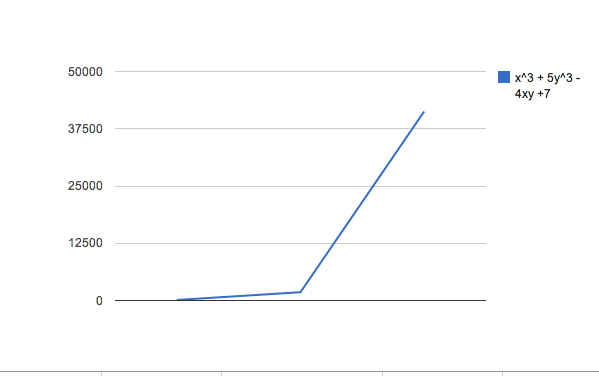
\includegraphics[width=90mm]{images/equa.png}
               \caption{The expression tested against, $ x^3 + 5y^3 - 4xy + 7 $}
                \label{equa}
        \end{center}
\end{figure}

\begin{figure}[!h]
        \begin{center}
		\scriptsize
		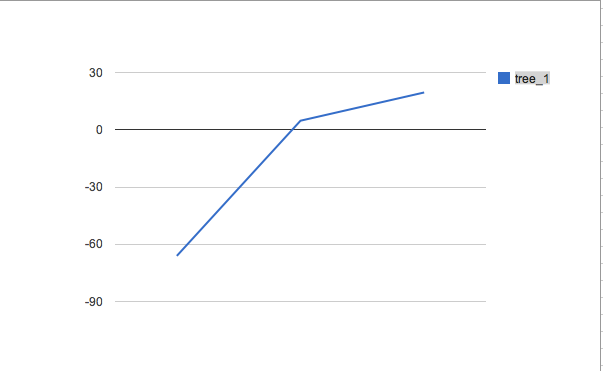
\includegraphics[width=90mm]{images/tree.png}
               \caption{Results from a random tree's expression}
                \label{tree}
        \end{center}
\end{figure}

\pagebreak


\section{Code}
\footnotesize
\subsection{Makefile}
\lstinputlisting{src/Makefile}

\subsection{main.h}
\lstinputlisting{src/main.h}

\subsection{main.cpp}
\lstinputlisting{src/main.cpp}

\subsection{tree\_node.h}
\lstinputlisting{src/tree_node.h}

\subsection{tree\_node.cpp}
\lstinputlisting{src/tree_node.cpp}

\subsection{tree.h}
\lstinputlisting{src/tree.h}

\subsection{tree.cpp}
\lstinputlisting{src/tree.cpp}

\subsection{test.h}
\lstinputlisting{src/test.h}

\subsection{test.cpp}
\lstinputlisting{src/test.cpp}


\end{document}
